\subsection{Data Collection/Synthesis}
The research aim to apply the developed deep learning models on two different datasets: one real-world dataset and another one from simulation of a multi-step supply chain. The synthesized dataset will have significant variability and random noises. The real world dataset should come from a renowned supplier's supply chain. 
Due to the implications connected with sharing industry data, the real world datasets may not be very effective in this study. As an alternative the synthesized datasets come handy to develop and evaluate the models.

For every ML/DL applications, several preprocessing steps are employed to process raw data. These methods include data cleaning, transforming operation, normalization, feature engineering etc. There is no single preprocessing strategy that works well on every applications. One has to find the best sequence of operations to suit his needs\cite{kotsiantis2006data}. 


\subsection{Model Implementation}

Generally, most SC forecasting problems are uni-variate. These uni-variate time series forecasting problem can be modeled as a supervised learning problems as follows:

$$ y = f(x); \text{where $x$ is previous demand data, and $y$ is the forecast output.} $$
Uni-variate time series datasets need restructuring to be modeled as a supervised learning problem. A well established method of restructuring is \textbf{windowing}. In this approach, fixed sized windows are created from previous time steps and the next immediate time step is considered as the output. These pairs of data are fed into the neural network for training. There exists variety of deep learning techniques for forecasting application. 

\noindent The state-of-the-art neural network architectures include:
\begin{enumerate}
    \item{Artificial Neural Networks(ANNs)}
    \item{Convolutional Neural Networks (CNNs)}
    \item{Recurrent Neural Networks(RNNs)}
    \item{Long-short Term Memory(LSTMs)}
\end{enumerate}

Many researchers have also applied hybrid-models for forecasting applications. Such models include:
\begin{enumerate}
    \item{CNN-RNN}
    \item{CNN-LSTM}
\end{enumerate}

Applying these methods after decomposing the demand series into several IMFs is also a popular approach. Another approach is inclusion of auxiliary variables into the model to increase forecasting accuracy. Finally I intend to study the transfer learning approach on this regard. This approach would be novel in demand forecasting.

Deep learning models possess many hyper-parameters. Hence it is mandatory to tune those parameters to achieve best results from the models. Trying random values for the parameters and coarse to fine sampling scheme are widely used for optimization. 

\subsection{Benchmarking}
The thesis will include the benchmarks of costs and benefits of applying these models for supply chain demand forecasting. Specifically, I suggest the followings: \\

Firstly, \textbf{RMSE} and \textbf{MAPE}. These will evaluate the forecasting error margins that the SC will have to endure.

Secondly, \textbf{data costs}. Generally DL models improve as the data volumes increases. But data collections and storage have costs connected to them. Thus the organizations have to face cost-accuracy trade-off.

Finally, \textbf{overall application impact}. For a new application like this a SC has to go through many challenges. At last these implications and expectancies will be discussed. 


\begin{figure}
    \centering
    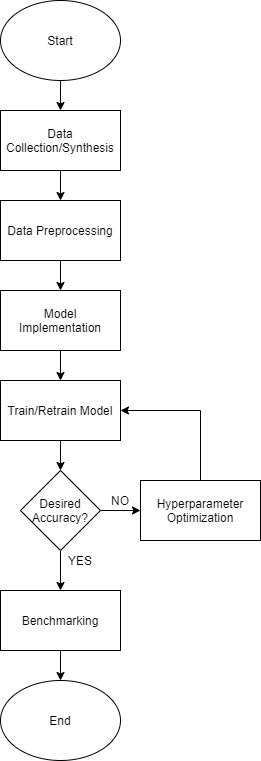
\includegraphics[scale=0.8]{flow-Page-1.jpg}
    \caption{Research Methodology Flow Chart}
    \label{fig:flowchart}
\end{figure}
